\documentclass[11pt]{article}
\usepackage[paper=a4paper,left=25mm,right=25mm,top=25mm,bottom=25mm]{geometry}
\usepackage[utf8]{inputenc}
\usepackage[german]{babel}
\usepackage{float}
\usepackage{graphicx}
\usepackage{wrapfig}
\usepackage{gensymb}
\usepackage{multirow}
\usepackage[center]{caption}
\usepackage{lscape}
\usepackage{eqnarray}
\usepackage{xcolor}
\usepackage{colortbl}
\usepackage{url}
\usepackage{hyperref}
\usepackage{varioref}
\usepackage{appendix}
\usepackage{subcaption}
\usepackage{mathtools}
\usepackage{amsmath}
\usepackage{amssymb}
\usepackage{siunitx}
\usepackage{chemformula}
\usepackage{cleveref}
\usepackage{import}
\usepackage{pdfpages}
\usepackage{tikz}
\usepackage{adjustbox}
\usepackage{bm}
\usepackage[normalem]{ulem}


\begin{document}

\pagenumbering{gobble} %Verhindert die Seitennummerierung auf der Titelseite und Aufgabenbaltt

%--------Deckblatt Versuchsprotokoll----------%
\import{chapters/}{Deckblatt}
\pagebreak
%---------------------------------------------%

%--------Aufgabenblatt----------%
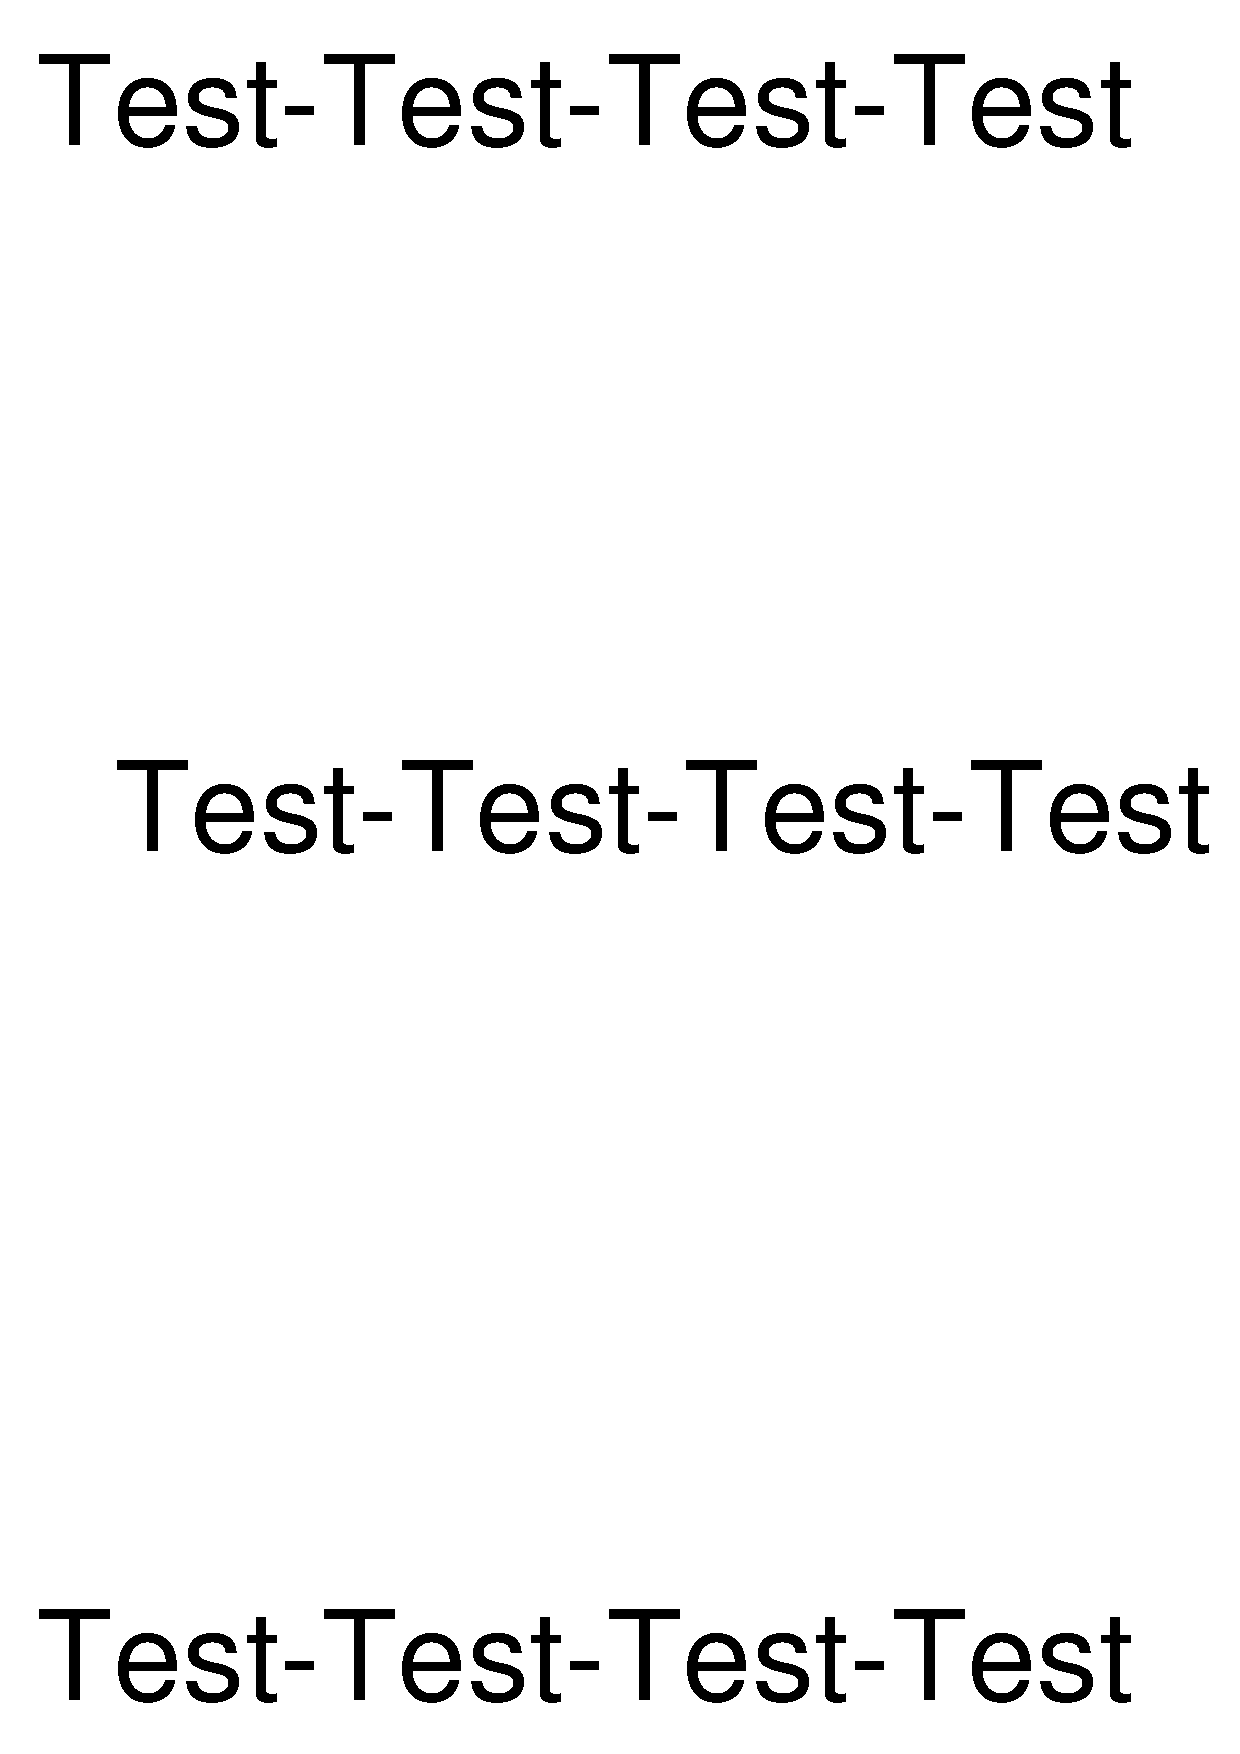
\includepdf[pages=-]{include/Aufgabenblatt.pdf}
\pagebreak
%-------------------------------%

%--------Inhaltsverzeichnis und Abbildungsverzeichnis----------%
\setcounter{section}{-1} 
% Bei "\setcounter{section}{-1}" erhält die Einführung die Kapitelnummer "0";
% Dies kann praktisch sein, um die Kapitelnummer mit den Aufgabennummern der Versuche gleich zu halten.
% Bei "\setcounter{section}{0}" startet das Inhaltsverzeichnis bei "1".
\tableofcontents % Erstellt ein Inhaltsverzeichnis
%\vspace{50px}   
%\listoffigures  % Erstellt ein Abbildungsverzeichnis
%\vspace{50px}   
%\listoftables  % Erstellt ein Tabellenverzeichnis
\pagebreak
%--------------------------------------------------------------%

\pagenumbering{arabic} % Ab hier beginnt die Seitennummerierung
\setcounter{page}{1}   % mit Seitenzahl 1.

%--------Inhalt der Kapitel----------%
\import{chapters/}{Einführung}
\pagebreak

\import{chapters/}{01}
\pagebreak

\import{chapters/}{02}
\pagebreak

\import{chapters/}{03}
\pagebreak

\import{chapters/}{04}
\pagebreak
%------------------------------------%

%--------Quellen----------%
\import{chapters/}{Quellen}

\pagebreak
%-------------------------%

%--------Anhang (Messprotokoll)----------%
\section{Messprotokoll}
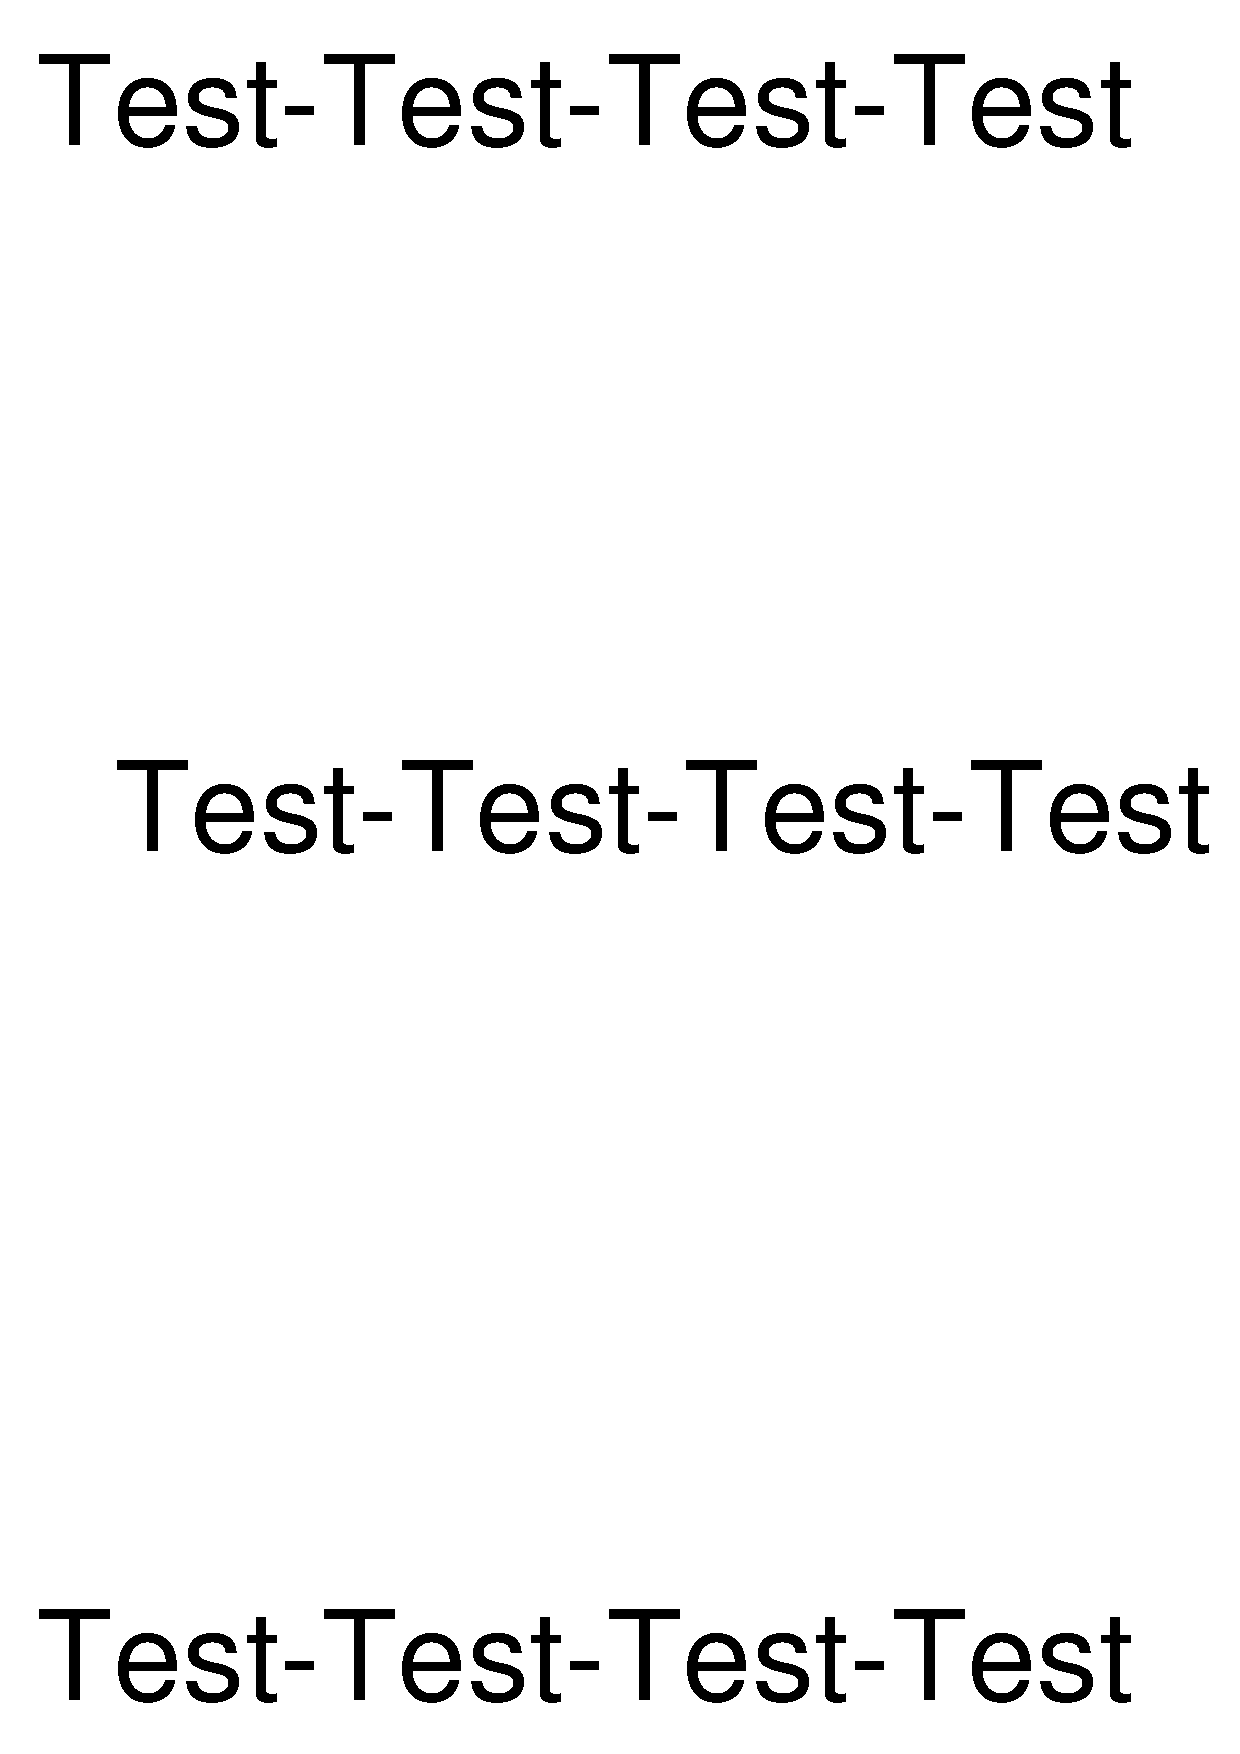
\includepdf[pages=-]{include/Messprotokoll.pdf}
%------------------------%


\end{document}